% Shared preamble of the two Lodos v2 manuals, collision_detection.tex and contact_dynamics.tex.
%
% The notation and the palette follow the contact tutorial (papers/contact_tutorial.pdf):
% plain math, q-dot and q-ddot the generalized velocity and acceleration, v a contact
% velocity, G the Delassus matrix, R the regularization, gamma_n the stabilization and
% Gamma the de Saxce correction.
%
% tex2md.py turns each manual into Markdown. It understands the commands and environments
% defined here and the standard ones the manuals use; keep math free of custom macros, so
% that it reads the same in both.

\documentclass[11pt,a4paper]{article}

% --- Fonts ---
\usepackage[T1]{fontenc}
\usepackage[utf8]{inputenc}
\usepackage{amsmath}
\usepackage{libertine}
\usepackage[libertine]{newtxmath}
\usepackage[varqu,scaled=0.92]{zi4}
\usepackage{microtype}

% --- Page ---
\usepackage[a4paper,margin=24mm,top=22mm,bottom=24mm]{geometry}
\setlength{\parindent}{0pt}
\setlength{\parskip}{5pt plus 1pt}
\linespread{1.04}

% --- Colours: the tutorial's ---
\usepackage[table]{xcolor}
\definecolor{ourblue}{rgb}{0.368,0.507,0.71}
\definecolor{ourorange}{rgb}{0.881,0.611,0.142}
\definecolor{ourgreen}{rgb}{0.56,0.692,0.195}
\definecolor{ourred}{rgb}{0.923,0.386,0.209}
\definecolor{ourviolet}{rgb}{0.528,0.471,0.701}
\definecolor{ourbrown}{rgb}{0.772,0.432,0.102}
\definecolor{ourazure}{rgb}{0.364,0.619,0.782}
\definecolor{ourgray}{RGB}{102,88,84}
\definecolor{ourgray2}{RGB}{124,124,115}
\definecolor{ourlightgray2}{RGB}{194,194,189}
\definecolor{ourdarkblue2}{RGB}{5,97,164}
\definecolor{codebg}{RGB}{246,247,249}

% --- Headings: sans, as the tutorial's ---
\usepackage[scaled=0.92]{helvet}
\usepackage{titlesec}
\titleformat{\section}{\sffamily\bfseries\Large}{\thesection}{0.6em}{}
\titleformat{\subsection}{\sffamily\bfseries\large}{\thesubsection}{0.6em}{}
\titleformat{\subsubsection}{\sffamily\bfseries\normalsize}{\thesubsubsection}{0.6em}{}
\titleformat{\paragraph}[runin]{\sffamily\bfseries\normalsize}{}{0pt}{}[.]
\titlespacing*{\section}{0pt}{14pt plus 3pt}{6pt}
\titlespacing*{\subsection}{0pt}{11pt plus 2pt}{4pt}
\titlespacing*{\subsubsection}{0pt}{9pt plus 2pt}{3pt}
\titlespacing*{\paragraph}{0pt}{6pt plus 1pt}{0.6em}

% --- Figures, tables, lists ---
\usepackage{graphicx}
\usepackage{booktabs,tabularx,array,longtable}
\newcolumntype{L}[1]{>{\raggedright\arraybackslash}p{#1}}
\newcolumntype{R}[1]{>{\raggedleft\arraybackslash}p{#1}}
\newcolumntype{Y}{>{\raggedright\arraybackslash}X}
\renewcommand{\arraystretch}{1.12}
\usepackage[font=small,labelfont={bf,sf}]{caption}
\usepackage{enumitem}
\setlist{itemsep=1pt,topsep=3pt,parsep=1pt,leftmargin=1.4em}
\setlist[itemize]{label={\color{ourblue}\textbullet}}

% --- Boxes: the tutorial's equation box, and the implementation notes ---
\usepackage[most]{tcolorbox}
\newtcolorbox{equationbox}[1]{
    enhanced, sharp corners, colback=white, colframe=black!60, boxrule=0.8pt,
    top=0.6em, attach boxed title to top left={xshift=-1mm, yshift=-5mm, yshifttext=-1mm},
    boxed title style={sharp corners, size=small, colback=black!60, colframe=black!60},
    fonttitle=\bfseries\sffamily, title=#1}
% "In the code": where a section's theory lives in the repository.
\newtcolorbox{codebox}{
    enhanced, sharp corners, colback=codebg, colframe=ourblue, boxrule=0pt,
    leftrule=2.2pt, left=6pt, right=6pt, top=3pt, bottom=3pt, before skip=6pt, after skip=6pt,
    fontupper=\small}
% A note with a title of its own (a finding, a caveat, a rule).
\newtcolorbox{notebox}[1]{
    enhanced, breakable, sharp corners, colback=ourorange!6, colframe=ourorange, boxrule=0pt,
    leftrule=2.2pt, left=6pt, right=6pt, top=3pt, bottom=3pt, before skip=6pt, after skip=6pt,
    fontupper=\small, title={#1}, coltitle=black, fonttitle=\bfseries\sffamily\small,
    colbacktitle=ourorange!6, attach title to upper={.\ }}

% --- Code ---
\usepackage{needspace}
\usepackage{listings}
\lstdefinestyle{lodos}{
    basicstyle=\ttfamily\small, backgroundcolor=\color{codebg}, frame=single,
    framerule=0pt, rulecolor=\color{codebg}, xleftmargin=4pt, xrightmargin=4pt,
    aboveskip=6pt, belowskip=6pt, columns=fullflexible, keepspaces=true,
    showstringspaces=false, breaklines=true, breakatwhitespace=false,
    keywordstyle=\color{ourdarkblue2}, commentstyle=\color{ourgray2}\itshape,
    stringstyle=\color{ourbrown}, upquote=true}
\lstset{style=lodos, language=Python}
% Identifiers and paths: typewriter, breaking at dots, underscores and slashes.
\usepackage[obeyspaces,spaces]{url}
\DeclareUrlCommand\codeurl{\urlstyle{tt}}
% Robust, so that it survives captions and tables (moving arguments).
\DeclareRobustCommand{\code}[1]{\codeurl{#1}}
\renewcommand{\UrlBreaks}{\do\.\do\_\do\/\do\,\do\(\do\=\do\-}

% --- TikZ, plots, algorithms ---
\usepackage{tikz}
\usetikzlibrary{arrows.meta,positioning,calc,fit,backgrounds,decorations.pathreplacing,shapes.geometric}
\usepackage{algorithm}
\usepackage{algpseudocode}
\algrenewcommand\algorithmicrequire{\textbf{Input:}}
% One hyperref anchor per line of every algorithm, not one per line number.
\makeatletter\providecommand{\theHALG@line}{}\renewcommand{\theHALG@line}{\thealgorithm.\arabic{ALG@line}}\makeatother
\algrenewcommand\algorithmicensure{\textbf{Output:}}

% --- Links and references ---
\usepackage[colorlinks=true,allcolors=ourdarkblue2,breaklinks=true,bookmarksnumbered=true]{hyperref}
\usepackage[capitalise,noabbrev]{cleveref}
\crefname{section}{Section}{Sections}
\crefname{subsection}{Section}{Sections}
\crefname{subsubsection}{Section}{Sections}
\crefname{appendix}{Appendix}{Appendices}
\crefname{equation}{Eq.}{Eqs.}
\crefname{figure}{Figure}{Figures}
\crefname{table}{Table}{Tables}
\crefname{algorithm}{Algorithm}{Algorithms}
\creflabelformat{equation}{#2(#1)#3}

% --- Title block: \manualtitle{title}{subtitle}{the line under it} ---
\newcommand{\manualtitle}[3]{%
  {\sffamily\bfseries\huge #1\par}\vspace{4pt}%
  {\sffamily\Large\color{ourgray} #2\par}\vspace{6pt}%
  {\small\color{ourgray2} #3\par}\vspace{8pt}%
  {\color{ourblue}\rule{\linewidth}{1.2pt}}\par\vspace{4pt}}

\newcommand{\micro}{\textmu}

\begin{document}

\manualtitle{Lodos v2: Where the Speed-up Comes From}{A stage-by-stage profile of the MuJoCo Warp comparison, and why Lodos's collision pipeline is faster}{Lodos v2 as of 2026-11-10. A measurement report on three scenes of the benchmark in \code{bench/lodos_mjwarp/} (\code{papers/lodos_v2.pdf}, Table 1), on top of the manual \emph{Collision Detection} (\code{docs/collision_detection.pdf}), whose pipelines it measures, and the guide \emph{Performance Tuning} (\code{docs/performance_tuning.pdf}). The tools and the record of every number are in \code{bench/lodos_mjwarp/profile/}. Built from \code{docs/manual/}.}

\paragraph{About this document}
The benchmark of \code{bench/lodos_mjwarp/} runs Lodos's mj mode against MuJoCo Warp as Newton runs it, and reports each one's throughput at the batch size where it is highest. On the three scenes measured here, Lodos's lead is 33--38$\times$ on the NIST threading task, and 5.2--8.3$\times$ and about 6$\times$ on five armadillos dropped into a box, as surfaces and as hulls. This report asks where those factors come from: which parts of the step, how much each, and, for collision detection, why. It answers by timing every stage of both simulators inside the benchmark's own runs, then the kernels inside the stages, and by counting what each pipeline produces along the way.

All numbers are measured on an RTX 4080 (16\,GiB) on 2026-11-10, the step captured as one CUDA graph and replayed, at the batch size stated. A world-step is a step of one world: times are given per world-step, the step's time divided by the batch size $B$, in microseconds.

\setcounter{tocdepth}{1}
\tableofcontents

\section{The short version}\label{sec:short}

\begin{enumerate}
\item \textbf{Collision detection is the largest source of the speed-up.} At each simulator's best batch size, Lodos's collision is 59$\times$ faster per world-step on the threading, 6.5$\times$ on the armadillos as surfaces and 10$\times$ as hulls, and accounts for 92\%, 41\% and 62\% of the time Lodos saves (\cref{sec:where}). At equal batch size it is 38$\times$, 6.6$\times$ and 7.6$\times$.
\item \textbf{Three mechanisms make it faster} (\cref{sec:why}):
  \begin{itemize}
  \item \emph{cheap conservative filters before any exact evaluation}: of 16\,064 vertex candidates per world on the threading, 1\,566 survive the box and tile tests, 306 the voxel lookup, and only those meet the spline field;
  \item \emph{contacts only where bodies penetrate}: Newton's pipeline also makes every contact within a detection gap, which MuJoCo Warp then mostly ignores (of 71.5 contacts per world on the armadillos, about 5 become constraints);
  \item \emph{the previous step, reused}: on the hulls, Lodos's narrowphase settles 86\% of its pairs from a per-world cache and runs GJK on 9.5 pairs per world, where Newton runs GJK and MPR on all of its 276.
  \end{itemize}
\item \textbf{The solve's speed-up is mostly a contact-count effect} (\cref{sec:solve}). Both simulators solve problems of similar size, with similar iteration counts, yet MuJoCo Warp's solve is 3.5--5.3$\times$ slower at equal batch size. One kernel, the elliptic cones' Hessian update, is 62--77\% of it, and its cost grows with every contact handed to MuJoCo Warp, active or not. On the threading, Lodos's fused Newton solve adds a 6$\times$ of its own.
\item \textbf{Batch size} (\cref{sec:batch}). Lodos's cost per world-step keeps falling up to $B$ = 8\,192, where MuJoCo Warp's best is 1\,024--2\,048: about half of the threading's factor comes from there.
\item \textbf{The threading's baseline collides two fixed bodies} (\cref{sec:weld}). Newton's importer makes the bolt and the board bodies of their own, fixed to the world, and collides them every step, which MuJoCo never does. Leaving such pairs out makes MuJoCo Warp 1.74$\times$ faster on that scene: Lodos's lead there becomes 19$\times$ (per contact) and 22$\times$ (ray groups) at the best batch sizes, and 10--11$\times$ at equal batch size, instead of 33--38$\times$ and 18--19$\times$.
\end{enumerate}

\begin{figure}[t]
\centering
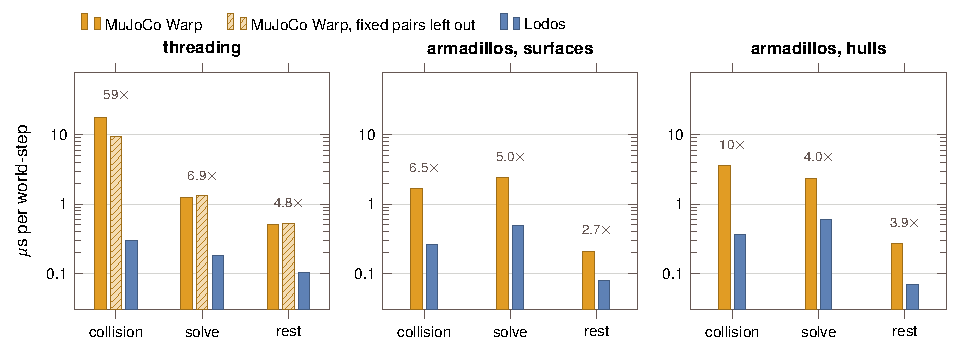
\includegraphics[width=\linewidth]{fig/fig_speedup.pdf}
\caption{Time per world-step by part of the step, each simulator at the batch size the benchmark found best (Lodos per contact: $B$ = 8\,192, 4\,096, 8\,192; MuJoCo Warp: 1\,024, 2\,048, 2\,048), log scale. ``Rest'' is the rigid-body pass and integration, the constraint assembly and the tracking. The labels are Lodos's speed-up on each part. On the threading, the hatched bars are MuJoCo Warp with the pairs of bodies fixed to the world left out (\cref{sec:weld}).}
\label{fig:speedup}
\end{figure}

\section{What was measured}\label{sec:setup}

\subsection{The benchmark}\label{sec:bench}

\code{bench/lodos_mjwarp/} (its \code{README.md}) compares two simulators on the same scenes, solver settings and starts:

\begin{itemize}
\item \textbf{Lodos} in its mj mode, at the viewer's defaults for the scene, with the implicitfast integrator and its contacts reduced, under each kind of contact group: per contact, cone and ray (collision manual, \emph{Contacts into the solver}). Each configuration's capacities are measured by the benchmark's tune phase (each 1.5 times its peak over 16 starts), and its ab phase keeps an execution option where it is 3\% faster: the fused Newton solve on the threading, no shared Hessian on the hulls, the default on the armadillos as surfaces.
\item \textbf{MuJoCo Warp} as Newton 1.7.0 runs it: Newton's collision pipeline (its broadphase over the pairs its filters allow, its narrowphase, and its reduction of mesh contacts, all at their defaults), the contacts converted into MuJoCo Warp's arrays, and MuJoCo Warp 3.15's step (\code{SolverMuJoCo} with \code{use_mujoco_contacts=False}), at Lodos's solver settings: Newton's method, the elliptic cone, the same iteration and tolerance budgets, every contact's solref the same.
\end{itemize}

The benchmark's ladder doubles each configuration's batch size from 64 until its throughput drops, and \code{report/best.json} records the best. Every run here is at a batch size from that file, from the benchmark's own starts and recorded controls, over the scene's whole duration.

\subsection{The scenes}\label{sec:scenes}

\begin{table}[t]
\centering
\caption{The three scenes (\code{bench/lodos_mjwarp/common.py}), as each simulator collides them. Newton's gap is the distance within which its pipeline makes contacts (\cref{sec:gap}): 1\% of the scene's body size for the shapes without a gap of their own (\code{newton_scene.gap_of}), and the scene's own gaps on the threading's parts and board.}
\label{tab:scenes}
\small
\begin{tabularx}{\linewidth}{@{}L{27mm}YYY@{}}
\toprule
scene & what & Lodos collides & Newton collides \\
\midrule
\textbf{threading} \code{nist_threading_m8} & A Franka hand threading an M8 nut onto its bolt on the NIST board, replaying a recorded control sequence. 15 dofs; 1.25\,ms steps, 5\,s (4\,000 steps). & 5 surfaces (the board, the bolt, the nut, two finger pads), 6 directional pairs: the nut's 3\,235 vertices on the other four fields, the bolt's 1\,562 on the pads'. The MJCF's other geoms through MJWarp's pipeline. & Isaac Lab's own collision meshes of the nut and the bolt with SDFs at its demo's settings; the board and the pads as boxes. Gap 5\,mm on the parts, 10\,mm on the board. \\
\textbf{armadillos, surfaces} \code{arm_walled_5_sdf} & Five armadillos dropped into a walled box. 30 dofs; 2\,ms steps, 3\,s (1\,500 steps). & 5 armadillo surfaces of 451 vertices and 5 planes: 45 directional pairs. & The same 451-vertex meshes, with SDFs at the bake's voxel size; the planes. Gap 2.6\,cm. \\
\textbf{armadillos, hulls} \code{arm_walled_5_polytope} & The same drop, each armadillo as its convex pieces. & MJWarp's pipeline (\code{lodos.col.prim}) with the exact hull narrowphase. & Newton's convex narrowphase: GJK, MPR, a contact manifold. Gap 2.6\,cm. \\
\bottomrule
\end{tabularx}
\end{table}

\Cref{tab:scenes} lists them. The armadillos as surfaces are the like-for-like comparison: both simulators collide the same meshes. On the threading the geometry differs, since Newton runs the parts as Isaac Lab's demo has it collide them (\code{viewer.scenes.nist.newton_shapes}), and on the hulls the two narrowphases differ but the pieces are the same.

\subsection{Hardware and software}\label{sec:versions}

An RTX 4080 (16\,GiB, driver 580.126.09, CUDA 13.0), with nothing else running on it but the desktop. Lodos: Warp 1.16.0, MuJoCo 3.14.0, Python 3.14 (\code{uv sync --locked --no-default-groups}). Newton: Newton 1.7.0, MuJoCo Warp 3.15.0, Warp 1.18.0, Python 3.12 (\code{viewer/newton/}'s environment).

\section{How it was measured}\label{sec:method}

\subsection{Stages inside the graph}\label{sec:tracer}

A stage's time is measured where the benchmark spends it: inside the captured step. \code{tracer.Tracer} wraps the step's stage functions (module attributes and instance methods) so that each records a CUDA timing event before and after itself. Captured, the events become nodes of the step's graph, which is otherwise the benchmark's: the same kernels in the same order. Every step of the run launches the graph, and at about 200 steps spread over the run (every 20th on the threading, every 7th on the armadillos) the host synchronizes and reads each stage's elapsed time and the workload counters. A run is the scene's whole duration, from the benchmark's starts, and each configuration is run twice: once with the benchmark's own graph, timed by wall clock (its throughput), once traced.

\begin{itemize}
\item \textbf{Lodos's stages} (\code{lodos_stages.py}): the rigid-body pass; MJWarp's collision (geom poses, broadphase, convex and primitive narrowphases, the exact hull narrowphase); Lodos's collision in its three functions (\code{broadphase_bbox}: poses, box test, tile filter and stage-1 compaction; \code{broadphase_sdf}: voxel prefilter and stage-2 compaction; \code{narrowphase_sdf}: spline evaluation, stage-3 compaction and the contacts); the contact dynamics (the reduction, the groups, \code{make_constraint}, the solve); integration; the tracking.
\item \textbf{Newton's stages} (\code{newton_stages.py}): its collision (shape boxes, broad phase, narrow phase); the parts of \code{SolverMuJoCo.step}: the controls and the state into MuJoCo Warp, the contact conversion, MuJoCo Warp's step (kinematics, \code{crb}, constraint assembly, velocity, actuation, acceleration, the solve, the implicit integration) and the state back; the state copy; the tracking.
\end{itemize}

\Cref{tab:categories} groups them into five parts that both simulators have. The traced step is within 3.5\% of the plain one at these batch sizes, and the benchmark's throughputs are reproduced within 0.3--5.5\% (\cref{tab:where}).

\begin{table}[t]
\centering
\caption{The parts of a step, as each simulator's stages are summed into them.}
\label{tab:categories}
\small
\begin{tabularx}{\linewidth}{@{}L{22mm}YY@{}}
\toprule
part & Lodos & MuJoCo Warp as Newton runs it \\
\midrule
collision & MJWarp's pipeline and the hull narrowphase, Lodos's pipeline, the contact reduction & Newton's collision pipeline, with its reduction \\
rigid body & the rigid-body pass, integration & the state into and out of MuJoCo Warp, kinematics, \code{crb}, velocity, actuation, acceleration, implicit integration \\
assembly & the export of Lodos's contacts and the groups, \code{make_constraint} & the contact conversion, \code{make_constraint} \\
solve & MJWarp's Newton solve, or the fused one & MuJoCo Warp's Newton solve \\
other & the tracking, gaps between stages & the same \\
\bottomrule
\end{tabularx}
\end{table}

\subsection{The share of the gap}\label{sec:share}

The speed-up is a ratio, $t^{\mathrm{MJW}} / t^{\mathrm{L}}$, of the two simulators' times per world-step. Where it comes from is told by the difference, which the parts $c$ of \cref{tab:categories} split additively. A part's share of the gap is
\begin{equation}\label{eq:share}
s_c = \frac{t^{\mathrm{MJW}}_c - t^{\mathrm{L}}_c}{t^{\mathrm{MJW}} - t^{\mathrm{L}}}, \qquad \sum_c s_c = 1,
\end{equation}
the fraction of the time Lodos saves that the part saves; it is negative for a part where Lodos is slower. A part can have the smaller ratio and the larger share if it costs more: on the armadillos as surfaces the solve is 5.0$\times$ faster and collision 6.5$\times$, but the solve takes 55\% of the gap because MuJoCo Warp spends 2.41\,\micro s solving and 1.68\,\micro s colliding. Two caveats go with every share here. At the best batch sizes it includes what the batch size does (\cref{sec:batch}). And the parts are not independent: a pipeline that hands the solve fewer contacts makes the solve cheaper too (\cref{sec:solve}).

\subsection{Kernels, counts, and the other runs}\label{sec:kernels}

\begin{itemize}
\item \textbf{Equal batch size}: Lodos again at MuJoCo Warp's best batch size, per contact and with ray groups.
\item \textbf{Kernels} (\code{collision_kernels.py}, \code{solve_kernels.py}): the benchmark's graph runs the scene, and at 8 steps spread over the run the collision stages, or a whole forward pass, run once more uncaptured under Warp's CUDA activity timing (\code{wp.timing_begin}). A stage recomputes its outputs from the poses, so the run is not changed. For the solve, the timing is stopped and restarted around the solve call, to keep its kernels apart. Uncaptured kernels are timed by events around each launch; their sums agree with the graph's stage times within 7\%.
\item \textbf{Censuses}: Newton's triangle pairs and contacts, counted per pair of shapes (\code{newton_pairs.py}); the hull narrowphase's path counters and the broadphase's pairs (\code{lodos_hybrid.py}, the collision manual's \code{HybridNarrowphase.stats}).
\item \textbf{Fixed pairs left out}: MuJoCo Warp on the threading with the shape pairs of bodies fixed to the world filtered (\code{newton_stages.py --weld-filter}, \cref{sec:weld}).
\end{itemize}

\section{Where the time goes}\label{sec:where}

\begin{table}[t]
\centering
\caption{Time per world-step by part (\micro s), each configuration at the batch size the benchmark found best. World-steps per second as measured here, the benchmark's in brackets; the parts are the traced step's (\cref{sec:tracer}). The cone groups, between per contact and ray on both surface scenes, are in \code{results.json}.}
\label{tab:where}
\small
\begin{tabularx}{\linewidth}{@{}Yrrrrrrrr@{}}
\toprule
configuration & $B$ & world-steps/s & total & collision & solve & rigid body & assembly & other \\
\midrule
\multicolumn{9}{l}{\emph{threading}} \\
Lodos, per contact & 8\,192 & 1.72M (1.74M) & 0.586 & 0.301 & 0.182 & 0.061 & 0.037 & 0.006 \\
Lodos, ray groups & 8\,192 & 1.94M (1.97M) & 0.531 & 0.310 & 0.060 & 0.063 & 0.090 & 0.009 \\
MuJoCo Warp & 1\,024 & 51.5k (52.0k) & 19.42 & 17.66 & 1.255 & 0.299 & 0.177 & 0.028 \\
\midrule
\multicolumn{9}{l}{\emph{armadillos, surfaces}} \\
Lodos, per contact & 4\,096 & 1.22M (1.24M) & 0.821 & 0.258 & 0.484 & 0.053 & 0.022 & 0.004 \\
Lodos, ray groups & 8\,192 & 1.94M (1.97M) & 0.518 & 0.273 & 0.174 & 0.041 & 0.027 & 0.003 \\
MuJoCo Warp & 2\,048 & 235k (238k) & 4.298 & 1.680 & 2.408 & 0.127 & 0.069 & 0.014 \\
\midrule
\multicolumn{9}{l}{\emph{armadillos, hulls}} \\
Lodos, per contact & 8\,192 & 967k (985k) & 1.024 & 0.363 & 0.592 & 0.039 & 0.028 & 0.003 \\
MuJoCo Warp & 2\,048 & 154k (163k) & 6.262 & 3.617 & 2.374 & 0.136 & 0.121 & 0.014 \\
\bottomrule
\end{tabularx}
\end{table}

\Cref{tab:where} and \cref{fig:speedup} give the parts; \cref{tab:share} the speed-up on each and its share of the gap.

\begin{table}[t]
\centering
\caption{Lodos's speed-up on each part, with its share of the gap (\cref{eq:share}) in brackets; at the best batch sizes ($B$ Lodos / MuJoCo Warp), and with Lodos at MuJoCo Warp's. ``With Lodos's collision'' is the speed-up that would remain if MuJoCo Warp's collision cost what Lodos's does.}
\label{tab:share}
\small
\begin{tabularx}{\linewidth}{@{}Yrrrrr R{19mm}@{}}
\toprule
scene, Lodos's groups & $B$ & speed-up & collision & solve & rigid body & with Lodos's collision \\
\midrule
\multicolumn{7}{l}{\emph{each at its best batch size}} \\
threading, per contact & 8\,192 / 1\,024 & 33.1$\times$ & 58.7$\times$ (92\%) & 6.9$\times$ (6\%) & 4.9$\times$ & 3.5$\times$ \\
threading, ray & 8\,192 / 1\,024 & 36.6$\times$ & 56.9$\times$ (92\%) & 21.0$\times$ (6\%) & 4.8$\times$ & 3.9$\times$ \\
surfaces, per contact & 4\,096 / 2\,048 & 5.2$\times$ & 6.5$\times$ (41\%) & 5.0$\times$ (55\%) & 2.4$\times$ & 3.5$\times$ \\
surfaces, ray & 8\,192 / 2\,048 & 8.3$\times$ & 6.1$\times$ (37\%) & 13.8$\times$ (59\%) & 3.1$\times$ & 5.6$\times$ \\
hulls, per contact & 8\,192 / 2\,048 & 6.1$\times$ & 10.0$\times$ (62\%) & 4.0$\times$ (34\%) & 3.5$\times$ & 2.9$\times$ \\
\midrule
\multicolumn{7}{l}{\emph{Lodos at MuJoCo Warp's batch size}} \\
threading, per contact & 1\,024 & 17.7$\times$ & 37.7$\times$ (94\%) & 5.3$\times$ (5\%) & 1.05$\times$ & 2.0$\times$ \\
threading, ray & 1\,024 & 17.2$\times$ & 39.5$\times$ (94\%) & 12.1$\times$ (6\%) & 1.09$\times$ & 2.0$\times$ \\
surfaces, per contact & 2\,048 & 4.6$\times$ & 6.6$\times$ (42\%) & 4.3$\times$ (55\%) & 1.7$\times$ & 3.1$\times$ \\
surfaces, ray & 2\,048 & 7.0$\times$ & 6.6$\times$ (39\%) & 10.9$\times$ (59\%) & 1.8$\times$ & 4.7$\times$ \\
hulls, per contact & 2\,048 & 4.9$\times$ & 7.6$\times$ (63\%) & 3.5$\times$ (34\%) & 1.9$\times$ & 2.5$\times$ \\
\bottomrule
\end{tabularx}
\end{table}

\begin{itemize}
\item \textbf{Collision and the solve are the step.} Together they are 95--97\% of MuJoCo Warp's step and 82--93\% of Lodos's per contact, and between them 96--98\% of the gap. The rigid-body pass and the assembly are each under 3\% of the gap everywhere.
\item \textbf{Collision decides the threading}: 92\% of the gap, a 59$\times$ faster stage. Given Lodos's collision, MuJoCo Warp would be within 3.5$\times$ of Lodos there. Half of its collision time is a pair of fixed bodies (\cref{sec:weld}); without it collision is still 85\% of the gap.
\item \textbf{The solve has the larger share on the armadillos as surfaces}, 55--59\%, and a third on the hulls, with ratios of 3.5--5.0$\times$ per contact. \Cref{sec:solve} finds that most of it, too, follows from the contacts each pipeline makes.
\item \textbf{The groups act on the solve}: ray groups cut it about 3$\times$ against per contact (0.06 against 0.18\,\micro s on the threading, 0.17 against 0.48 on the surfaces), at about the same collision cost and a little more assembly.
\end{itemize}

\section{Why Lodos's collision pipeline is faster}\label{sec:why}

\subsection{Cheap, conservative filters before the exact evaluation}\label{sec:funnel}

Lodos's pipeline (collision manual, \emph{The Lodos pipeline}) decides most of its candidates in groups and with single loads, and evaluates the spline field only on what is left:

\begin{enumerate}
\item the \emph{box test}, one oriented-box test per world and pair;
\item the \emph{tile filter}: the vertices of a surface are stored in Hilbert order and cut into tiles of 8, each with a bounding sphere; one lookup in the coarse voxel field at a tile's centre rejects all its vertices at once, with a margin that cannot reject a contact;
\item the \emph{voxel prefilter}: one voxel lookup per vertex of a surviving tile;
\item the \emph{narrowphase}: the tricubic spline, 64 coefficients and its gradient, on the survivors only, keeping the vertices where it is negative.
\end{enumerate}

Between stages the survivors are compacted, so that each launch runs over what the previous stage kept; a vertex is evaluated in the field's body frame from a small static array and one relative transform per pair, so no world-space vertex buffer is written; and a pair is directional, one part's vertices on the other's field, so a scene runs only the directions it needs (on the threading, the nut's vertices on the bolt's field, and not the reverse). \Cref{tab:funnel} measures the cascade.

Newton's pipeline takes the two surface scenes on two paths, both ending in one global reducer:

\begin{itemize}
\item \emph{mesh against mesh} (the nut on the bolt, an armadillo on another): each mesh's edges against the other's SDF, in both directions, culled per thread block by the edges' bounding spheres, with a contact wherever an edge comes within the gap;
\item \emph{mesh against a convex shape} (the threading's nut and bolt against the board and the pads): a BVH query for every mesh triangle that overlaps the shape's box, grown by the gap, then GJK or MPR on each triangle and the shape.
\end{itemize}

Every contact either path makes is written into a hash table that keeps, per pair of shapes and normal bin, the deepest contact and the most extreme ones (Newton's reduction, which Lodos's own reduction follows: collision manual, \emph{Contact reduction}).

\begin{table}[t]
\centering
\caption{What each pipeline produces, per world, mean over the sampled steps of the best-batch runs (Lodos per contact). Lodos's candidates are every vertex of every pair, counted once from the model; its tiles are 2\,012 and 2\,565 per world. MuJoCo Warp's active contacts are its constraint rows over 3, the rows of a contact on the elliptic cone at \code{condim} 3.}
\label{tab:funnel}
\small
\begin{tabularx}{\linewidth}{@{}Yrr@{}}
\toprule
& threading & armadillos, surfaces \\
\midrule
\multicolumn{3}{l}{\emph{Lodos}} \\
vertex candidates, all pairs & 16\,064 & 20\,295 \\
after the box and tile tests & 1\,566 (196 tiles) & 1\,223 (153 tiles) \\
after the voxel prefilter: spline evaluations & 306 & 33 \\
penetrating: contacts & 22.4 & 5.8 \\
handed to the solve, after the reduction & 11.9 & 5.8 \\
constraint rows & 35.6 & 17.3 \\
\midrule
\multicolumn{3}{l}{\emph{Newton}} \\
mesh triangles paired with a convex shape & 2\,761 & 0 \\
contacts into the reducer & 3\,095 & 107 \\
contacts out of the reducer & 225 & 71.5 \\
handed to MuJoCo Warp & 165 & 71.5 \\
constraint rows (active contacts) & 36.6 (12) & 15.8 (5) \\
\bottomrule
\end{tabularx}
\end{table}

\begin{itemize}
\item \textbf{The spline meets 2\% and 0.2\% of the candidates.} On the threading the box and tile tests remove 90\% of the vertices, eight at a time or a whole pair at once; on the armadillos the voxel lookup removes 97\% of what the tiles leave.
\item \textbf{Newton generates 138 and 18 times as many raw contacts} (3\,095 against 22.4, and 107 against 5.8) and reduces them afterwards, and on the threading it runs a narrowphase per mesh triangle: 2\,761 GJK or MPR queries per world.
\item \textbf{The solver sees about as many active contacts from either}: 12 against 11.9 on the threading, 5 against 5.8 on the armadillos. The difference above that line is in how much work it takes to find them.
\end{itemize}

\Cref{tab:collkernels} shows where each pipeline's time goes. On the threading, 12.3 of Newton's 18.0\,ms per step at $B$ = 1\,024 is the kernel that runs the narrowphase per mesh triangle and inserts the contacts into the reducer; Lodos's whole collision at that batch size takes 0.51\,ms. On the armadillos as surfaces, Newton's mesh--mesh kernel takes 2.7 of 3.4\,ms; Lodos's pipeline and reduction take 0.54\,ms, a third of it the reduction (\cref{sec:lodoscosts}).

\begin{table}[t]
\centering
\caption{The collision stages' largest kernels, ms per step at MuJoCo Warp's best batch size, mean of 8 states spread over the run, uncaptured (\code{collision_kernels.py}). Lodos's include its contact reduction, as \cref{tab:categories} does.}
\label{tab:collkernels}
\small
\begin{tabularx}{\linewidth}{@{}L{25mm}L{18mm}rY@{}}
\toprule
scene, $B$ & pipeline & total & largest kernels \\
\midrule
threading, 1\,024 & Lodos & 0.506 & spline evaluation 0.106, stage-1 scatter 0.069, tile filter 0.033, voxel prefilter 0.031, other SDF stages 0.096; reduction 0.082 (scoring 0.056); MJWarp's pipeline 0.089 \\
& Newton & 17.97 & mesh-triangle contacts into the reducer 12.29, mesh--mesh SDF 2.56, triangle overlap query 1.87, buffered reduction 0.60, export of the reduced contacts 0.43, other 0.22 \\
\midrule
surfaces, 2\,048 & Lodos & 0.535 & tile filter 0.087, stage-1 scatter 0.077, voxel prefilter 0.047, spline evaluation 0.034, other SDF stages 0.109; reduction 0.181 (filling its table 0.069, marking 0.050, scoring 0.049) \\
& Newton & 3.385 & mesh--mesh SDF 2.67, mesh--plane 0.40, export of the reduced contacts 0.18, buffered reduction 0.04, other 0.10 \\
\midrule
hulls, 2\,048 & Lodos & 0.915 & all-pairs broadphase 0.350, EPA 0.152, warm start and certificates 0.139, GJK 0.117, other 0.157 \\
& Newton & 7.666 & GJK 4.31, MPR 2.07, manifold 0.61, broadphase over the explicit pairs 0.52, other 0.15 \\
\bottomrule
\end{tabularx}
\end{table}

\subsection{Contacts only where bodies penetrate}\label{sec:gap}

Lodos makes a contact of a vertex only where the field is negative there, a penetration (collision manual, \emph{The stages}), and its hull narrowphase runs at zero gap. Newton's pipeline makes a contact wherever two shapes come within a \emph{gap} of each other: 1\% of the body size here, 2.6\,cm on the armadillos, and 5\,mm on the threading's parts and 10\,mm on its board, as the benchmark sets it (Newton's default is 10\,cm). MuJoCo Warp makes constraint rows only of the contacts inside the contact margin, so most of these are never rows: about 5 of the 71.5 contacts per world on the armadillos as surfaces, 11 of 58 on the hulls, 12 of 165 on the threading. In this pairing they are paid for three times: generated and reduced by the collision pipeline, converted, and looped over by the solve (\cref{sec:solve}).

\begin{notebox}{Not an error}
A gap is how Newton serves solvers and fast motion that need contacts before they touch, and its pipeline is shared by all of them. This report measures cost, not accuracy, and does not say that MuJoCo Warp would be as accurate without it.
\end{notebox}

\subsection{The previous step, reused: the hull scene}\label{sec:hulls}

On the armadillos as hulls neither simulator has an SDF. Lodos's pipeline is MJWarp's broadphase and its own exact hull narrowphase (collision manual, \emph{MJWarp's pipeline and the exact hull narrowphase}), which keeps each pair's minimizing feature from the last step in a per-world table and tries to certify the pair from it before running anything else: a separating axis that still separates, or a penetration axis whose depth a ball-containment test proves. \Cref{tab:hulls} counts what that does.

\begin{table}[t]
\centering
\caption{The hull scene per world, at $B$ = 2\,048, mean of 8 states spread over the run (\code{lodos_hybrid.py}; Newton's from its best-batch run).}
\label{tab:hulls}
\small
\begin{tabularx}{\linewidth}{@{}Yrr@{}}
\toprule
& Lodos & Newton \\
\midrule
candidate pairs from the broadphase & 75.7 & 276 \\
hull pairs found in the cache & 57.9 of 66.9 & -- \\
\quad certified separated / in contact from it & 54.6 / 2.7 & -- \\
pairs through GJK & 9.5 & 276 (and MPR) \\
pairs through EPA & 0.9 & -- \\
contacts & 6.9 & 58.3 (11 active) \\
\bottomrule
\end{tabularx}
\end{table}

\begin{itemize}
\item \textbf{A quarter of the candidates.} Lodos's broadphase runs at zero gap; Newton's boxes are grown by 2.6\,cm.
\item \textbf{Most pairs never reach GJK}: 82\% of them are certified separated from the cache, 4\% certified in contact. GJK runs on 9.5 pairs per world against Newton's GJK and MPR on 276, which take 6.4 of its 7.7\,ms (\cref{tab:collkernels}).
\item \textbf{Lodos's largest hull-scene kernel is its all-pairs broadphase}: 0.35 of 0.92\,ms.
\end{itemize}

\subsection{What is not the pipeline}\label{sec:notpipeline}

Two differences between the factors are the scenes', not the pipelines'. On the threading, Newton collides Isaac Lab's meshes of the parts and two boxes where Lodos collides its remeshed parts and four fields: the same physical contacts, other geometry. And half of Newton's collision there is a pair that should not be collided at all (\cref{sec:weld}). The armadillos as surfaces, where both collide the same meshes, give the cleanest measure of the pipelines: 6.5$\times$ at the best batch sizes and 6.6$\times$ at equal ones.

\section{Why the solve is faster}\label{sec:solve}

Both simulators solve with MuJoCo Warp's Newton method (Lodos's is adapted from MuJoCo Warp 3.14), on problems of about the same size: at the best batch sizes, 35.6 against 36.6 constraint rows per world on the threading, 17.3 against 15.8 on the surfaces, 20.1 against 32.8 on the hulls, in 2.8--3.5 iterations on average. Yet at equal batch size MuJoCo Warp's solve is 5.3$\times$, 4.3$\times$ and 3.5$\times$ slower. \Cref{tab:solve} splits one forward pass's solve into kernels.

\begin{table}[t]
\centering
\caption{The solve's kernels per forward pass, ms at MuJoCo Warp's best batch size, mean of 8 states spread over the run, uncaptured (\code{solve_kernels.py}; on the threading MuJoCo Warp with the fixed pairs left out, which does not change its contacts). Rows and iterations per world at those states, contacts per world from the best-batch runs (\cref{tab:funnel,tab:hulls}); JTCJ is \code{_update_gradient_JTCJ_dense}.}
\label{tab:solve}
\small
\begin{tabularx}{\linewidth}{@{}L{27mm}Yrrrrr@{}}
\toprule
scene, $B$ & simulator & contacts & rows & iterations & solve & of which JTCJ \\
\midrule
threading, 1\,024 & Lodos (fused) & 11.9 & 25.4 & 2.0 & 0.172 & -- \\
& MuJoCo Warp & 165 & 29.5 & 1.9 & 1.063 & 0.661 (62\%) \\
surfaces, 2\,048 & Lodos & 5.8 & 17.7 & 3.0 & 1.426 & 0.560 (39\%) \\
& MuJoCo Warp & 71.5 & 16.1 & 3.3 & 4.984 & 3.861 (77\%) \\
hulls, 2\,048 & Lodos & 6.8 & 20.5 & 3.0 & 1.832 & 0.673 (37\%) \\
& MuJoCo Warp & 58.3 & 33.5 & 3.0 & 4.899 & 3.231 (66\%) \\
\bottomrule
\end{tabularx}
\end{table}

\paragraph{One kernel} \code{_update_gradient_JTCJ_dense} adds the elliptic cones' blocks to the Hessian of Newton's method. It is launched with one thread per entry of the Hessian's lower triangle (465 at 30 dofs) and per block of contacts, and each thread loops over every contact handed to the solver, in every iteration; a contact outside the margin is skipped only after its world, the world's done flag, its dimension, distance and margin have been read (\code{mujoco_warp/_src/solver.py}). Its cost therefore grows with the contacts handed over, active or not. MuJoCo Warp is handed 165, 71.5 and 58 contacts per world, of which about 12, 5 and 11 are active; Lodos hands over 11.9, 5.8 and 6.8, all of them penetrating. The kernel is 7.6$\times$ and 5.6$\times$ slower per call in MuJoCo Warp on the two armadillo scenes. Charged at Lodos's time, MuJoCo Warp's solve would take 1.68 against Lodos's 1.43\,ms on the surfaces and 2.34 against 1.83 on the hulls: 1.2--1.3$\times$, mostly the mass-matrix product (\code{mul_m}, 0.31 against 0.05\,ms on the surfaces) and, on the hulls, the rows their manifolds add.

\paragraph{The fused solve} On the threading the benchmark's ab phase kept Lodos's fused Newton solve (companion manual \emph{Contact Dynamics}): Newton's iterations as one kernel per world, its data in the multiprocessor's shared memory. It takes 0.17\,ms where MuJoCo Warp's, a sequence of 63 launches, takes 1.06.

\begin{notebox}{What this means for the decomposition}
Most of the solve's share in \cref{tab:share} is collision's. The solve is as fast as the contacts it is handed allow, and the pipeline that hands it only penetrating contacts makes it 4--5$\times$ cheaper there.
\end{notebox}

\section{Batch size}\label{sec:batch}

Lodos's time per world-step keeps falling well past MuJoCo Warp's best batch size: from 1.10 to 0.59\,\micro s between $B$ = 1\,024 and 8\,192 on the threading, from 0.93 to 0.82 between 2\,048 and 4\,096 on the surfaces, from 1.28 to 1.02 between 2\,048 and 8\,192 on the hulls. MuJoCo Warp's throughput peaks at 1\,024 and 2\,048. The difference is a factor of 1.9 of the threading's 33$\times$ (17.7$\times$ at equal batch size), 1.1 and 1.25 on the armadillos. It is most of what separates the rigid-body passes: 1.05--1.9$\times$ at equal batch size, 2.4--4.9$\times$ at the best ones, MuJoCo Warp's including the conversion of the state to and from Newton's.

\section{The threading's baseline: two fixed bodies collide}\label{sec:weld}

\Cref{tab:census} counts which pairs of shapes give Newton's pipeline its work on the threading.

\begin{table}[t]
\centering
\caption{Newton's collision on the threading, per world, by pair of shapes (\code{shape@body}), mean of 8 states spread over the run at $B$ = 256 (\code{newton_pairs.py}). The nut's and the bolt's meshes are labelled \code{lodos_surface}.}
\label{tab:census}
\small
\begin{tabularx}{\linewidth}{@{}Yrr@{}}
\toprule
pair & mesh triangles paired & contacts out of the reducer \\
\midrule
bolt and board (\code{lodos_surface@bolt_m8}, \code{board_box@board}) & 1\,467 & 60.0 \\
nut and board & 531 & 24.2 \\
bolt and right pad & 467 & 3.7 \\
nut and right pad & 147 & 7.5 \\
bolt and left pad, nut and left pad & 31 & -- \\
bolt and nut (mesh--mesh) & -- & 125.1 \\
board and pads & -- & 1.8 \\
total & 2\,644 & 222.3 \\
\bottomrule
\end{tabularx}
\end{table}

In the scene's MJCF the bolt and the board are bodies without joints, welded to the world, and MuJoCo never collides two bodies welded to the same body; Lodos's scene has no such pair either. Newton's importer makes each a body of its own with a fixed joint to the world (as it does the arm's base, \code{link0}), and its pipeline pairs them: the bolt, whose lower part stands inside the board, against the board's box, in every step. That pair alone is 55\% of the triangles Newton pairs and 60 of its 222 contacts per world, which the conversion into MuJoCo Warp then drops: Newton makes 225 contacts per world in the best-batch run and MuJoCo Warp receives 165. They change nothing in the dynamics, and cost half of the collision.

\paragraph{Left out} \code{newton_stages.py --weld-filter} leaves out the shape pairs of bodies fixed to the world (63 shape pairs among the board, the bolt, the arm's base \code{link0} and the floor), as MuJoCo does:

\begin{itemize}
\item MuJoCo Warp's throughput rises from 51.5k to 89.8k world-steps/s (1.74$\times$), and is 89.6k at $B$ = 2\,048, so its best batch size stays 1\,024;
\item its collision falls from 17.66 to 9.37\,\micro s per world-step; Newton's triangle pairs from 2\,761 to 1\,294 per world, the contacts into its reducer from 3\,095 to 1\,609;
\item MuJoCo Warp's contacts, rows and iterations are unchanged: 165.4, 36.6 and 2.8 per world.
\end{itemize}

\begin{table}[t]
\centering
\caption{Lodos's speed-up on the threading against MuJoCo Warp as benchmarked and with the fixed pairs left out ($B$ = 1\,024 for MuJoCo Warp): the step's by throughput, collision's from the traced parts.}
\label{tab:weld}
\small
\begin{tabularx}{\linewidth}{@{}Yrrrr@{}}
\toprule
& \multicolumn{2}{c}{as benchmarked} & \multicolumn{2}{c}{fixed pairs left out} \\
Lodos's groups, $B$ & speed-up & collision & speed-up & collision \\
\midrule
per contact, 8\,192 (best) & 33.3$\times$ & 58.7$\times$ & 19.1$\times$ & 31.2$\times$ \\
ray, 8\,192 (best) & 37.7$\times$ & 56.9$\times$ & 21.6$\times$ & 30.2$\times$ \\
per contact, 1\,024 (equal) & 18.8$\times$ & 37.7$\times$ & 10.8$\times$ & 20.0$\times$ \\
ray, 1\,024 (equal) & 18.2$\times$ & 39.5$\times$ & 10.4$\times$ & 21.0$\times$ \\
\bottomrule
\end{tabularx}
\end{table}

\Cref{tab:weld} gives the threading's factors with the pair left out: 19--22$\times$ at the best batch sizes and 10--11$\times$ at equal ones, collision 85\% of the gap. The benchmark's threading should be rerun so, with an exclusion in the scene's Newton MJCF (\code{viewer.scenes.nist.newton_xml} already adds one, for the fingers) or with the filter \code{--weld-filter} applies, before its factor is quoted.

\section{Lodos's own costs}\label{sec:lodoscosts}

What the profile shows of Lodos's step, where it could be faster:

\begin{itemize}
\item \textbf{The contact reduction fills its whole table every step.} Its winner table is $(B, \min(n_{\mathrm{SEG}}, 16), 240)$ 64-bit slots, filled before every step's bids: 3\,840 slots (30\,kB) per world on the armadillos as surfaces, with their 45 segments, against 1\,440 on the threading's 6. There it costs 0.12\,\micro s per world-step at $B$ = 4\,096, 47\% of Lodos's collision and 15\% of its step, and keeps every contact it is given (5.8 in, 5.8 out). Filling only the rows the active segments take, or passing a segment with fewer contacts than it could keep, would recover most of it.
\item \textbf{The hulls' all-pairs broadphase} is the largest single kernel of the hull scene's collision, 0.35 of 0.92\,ms at $B$ = 2\,048, and at $B$ = 8\,192 it costs more than the whole hull narrowphase (0.175 against 0.165\,\micro s per world-step).
\item \textbf{The box and tile stage} is the largest of the SDF pipeline on the armadillos (0.083 of 0.137\,\micro s per world-step at $B$ = 4\,096), the narrowphase stage on the threading (0.119 of 0.225), most of it the spline evaluation.
\end{itemize}

\section{Limitations}\label{sec:limits}

\begin{itemize}
\item Three of the benchmark's fifteen scenes, one GPU, one run of each configuration (two passes over the scene's duration). The throughputs measured are 0.3--5.5\% below the benchmark's own; the largest difference is MuJoCo Warp on the hulls, whose run needed its \code{njmax} grown from the tuned 149 to 1\,192 rows per world after three overflows (a few worlds need more than 600 rows at times; the mean is 33).
\item Stage times are GPU time between events of the graph, sampled at about 200 steps of each run; kernel times are uncaptured, at 8 states. Both are means over a run whose load changes as the bodies settle.
\item The equal-batch comparisons are at MuJoCo Warp's best batch size only.
\item The parts of \cref{tab:categories} are a choice: Newton's state and contact conversions count as rigid body and assembly, and a part's share depends on that.
\item The gaps are the benchmark's choice (\cref{sec:gap}), and this report measures no accuracy: the two pipelines' contact sets differ in number and placement.
\end{itemize}

\section{Reproducing}\label{sec:reproduce}

\begin{codebox}
\textbf{In the code.} \code{bench/lodos_mjwarp/profile/}: \code{run_profiles.py} runs every measurement of this report into \code{results/lodos_mjwarp/profile/} (about 25 minutes on an RTX 4080, and about 10 more for the benchmark's prepare, tune and ab phases for the three scenes, which its \code{prepare} phase runs first); \code{summary.py} prints the tables and writes \code{results.json}, the record of every number here. \code{tracer.py}: the timing events inside the graph. \code{lodos_stages.py}, \code{newton_stages.py}: one configuration's two runs. \code{collision_kernels.py}, \code{solve_kernels.py}: the kernels. \code{newton_pairs.py}, \code{lodos_hybrid.py}: the censuses.
\end{codebox}

\begin{lstlisting}
.venv/bin/python bench/lodos_mjwarp/profile/run_profiles.py   # measure, about 35 min
.venv/bin/python bench/lodos_mjwarp/profile/summary.py        # tables, results.json
\end{lstlisting}

\end{document}
